\section{Training Dynamics and Cost}
\label{sec:results}

We logged training telemetry to Weights~\&~Biases for the fine-tuning runs:
train and validation loss, throughput, and peak memory. The capability and safety of the resulting models
are measured separately in \S\ref{sec:eval}. Fifteen runs have usable
histories; Table~\ref{tab:training-runs} lists
representative runs.

% AUTO-GENERATED by gen_wandb.py -- do not edit
\begin{table*}[t]
\centering
\caption{Representative LoRA runs from training telemetry. These are \emph{training} metrics only; no capability or safety evaluation was logged. `min' is the best validation loss reached.}
\label{tab:training-runs}
\footnotesize
\setlength{\tabcolsep}{5pt}
\begin{tabular}{llllrrr}
\hline
\textbf{Base model} & \textbf{Align.} & \textbf{Data} & \textbf{State} & \textbf{Steps} & \textbf{Train loss} & \textbf{Val loss (min)} \\
\hline
Qwen3-30B Instruct (8b) & aligned & defensive (instruction) & finished & 142 & 0.994$\to$0.613 & 1.268$\to$0.553 (0.548) \\
Qwen3-30B Instruct (8b) & aligned & defensive (instruction) & finished & 142 & 1.014$\to$0.617 & 1.313$\to$0.552 (0.548) \\
Qwen3-30B Instruct (8b) & abliterated & defensive (instruction) & finished & 142 & 1.133$\to$0.584 & 1.517$\to$0.492 (0.489) \\
Qwen3-30B Instruct (8b) & aligned & offensive (Code\_Vulns) & finished & 466 & 1.066$\to$0.299 & 2.665$\to$0.301 (0.248) \\
Qwen3-30B Instruct (8b) & abliterated & offensive (Code\_Vulns) & finished & 466 & 1.175$\to$2.018 & 2.853$\to$4.451 (0.228) \\
gpt-oss-120b (4-bit) & aligned & defensive (instruction) & killed & 31 & 2.76$\to$1.095 & 8.959$\to$0.954 (0.954) \\
Qwen3-4B Instruct & abliterated & offensive (Code\_Vulns) & finished & 233 & 1.448$\to$0.367 & 1.564$\to$0.354 (0.354) \\
Qwen3-4B Instruct & abliterated & offensive (Code\_Vulns) & killed & 336 & 0.88$\to$3.104 & 1.524$\to$3.086 (0.57) \\
\hline
\end{tabular}
\end{table*}


\paragraph{Convergence.}
On the defensive instruction data, the aligned Qwen3-30B Instruct model
converges smoothly to a best validation loss of $0.548$, and the offensive
Code\_Vulns objective on the same base reaches a lower best validation loss of
$0.248$ (Figure~\ref{fig:loss-dataset}), which is not surprising, as the offensive
targets are longer, more templated, and less varied than the diverse
defensive corpus. Lower loss here reflects easier fitting, not a safety or
capability claim.

\begin{figure}[t]
  \centering
  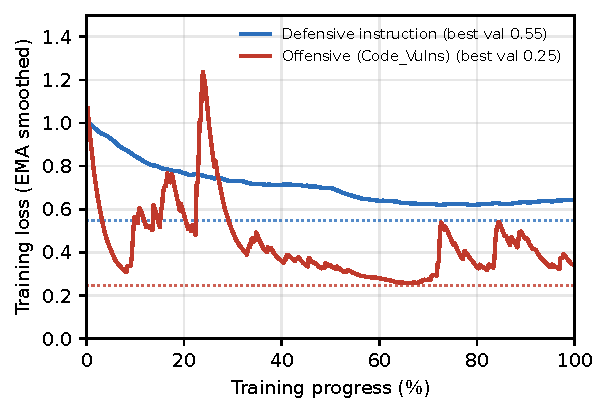
\includegraphics[width=\columnwidth]{fig_loss_dataset.pdf}
  \caption{Training loss (EMA smoothed) versus training progress on Qwen3-30B
  Instruct: defensive instruction data versus the offensive Code\_Vulns
  objective. The offensive
  objective fits to a lower loss.}
  \label{fig:loss-dataset}
\end{figure}

\paragraph{Aligned versus abliterated.}
Holding the data fixed (the formatted defensive set), the abliterated
Qwen3-30B base reaches a best validation loss of $0.489$, slightly below the
aligned Instruct model's $0.548$ (Figure~\ref{fig:loss-alignment}). Removing
refusal behavior does not impede (and marginally eases) fitting the
cybersecurity data. A de-aligned base is at least as amenable to this
fine-tuning as its aligned counterpart.

\begin{figure}[t]
  \centering
  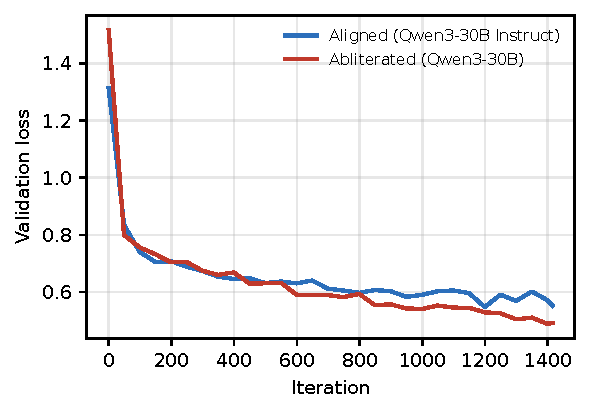
\includegraphics[width=\columnwidth]{fig_loss_alignment.pdf}
  \caption{Validation loss on identical defensive data: aligned versus
  abliterated Qwen3-30B. De-alignment does not hurt convergence.}
  \label{fig:loss-alignment}
\end{figure}

\paragraph{Training instability.}
Several offensive and abliterated runs did not converge cleanly. The
abliterated Qwen3-30B on Code\_Vulns diverged (validation loss rising from
$2.853$ to $4.451$), and an abliterated Qwen3-4B run destabilized late
(validation loss $1.524\to3.086$). These indicate that the offensive/de-aligned
configuration is more sensitive to schedule and length than the defensive one.

\paragraph{Cost on consumer hardware.}
The cost that matters to an adversary is wall clock time on owned hardware, not
the streaming rate. A complete offensive fine-tune of the 30B model finished in
$6.5$~hours over $8.0$~million tokens on a single Apple~Silicon machine; the 4B
model, run to a longer schedule, took up to $18.6$~hours and $25.2$~million
tokens (wall clock here tracks the iteration budget, not model size). Throughput
was $275$--$740$ tokens per second within $34.6$--$79.1$\,GB of memory
(Table~\ref{tab:training-cost}); the $120$B model was the slowest and most
memory-hungry, at about $275$ tokens per second and $79.1$\,GB. There is no
cloud bill and no costs beyond hardware and electricity: one desktop left running for
an afternoon or overnight is the entire capital requirement.

% AUTO-GENERATED by gen_wandb.py -- do not edit
\begin{table}[t]
\centering
\caption{LoRA fine-tuning throughput and peak memory on a single Apple~Silicon machine. Ranges span the usable runs for each base model.}
\label{tab:training-cost}
\small
\setlength{\tabcolsep}{3pt}
\begin{tabular}{lrr}
\hline
\textbf{Base model} & \textbf{Tok/s} & \textbf{Peak (GB)} \\
\hline
Qwen3-4B Instruct & 468--568 & 34.6 \\
gpt-oss-120b (4-bit) & 275--309 & 79.1 \\
Qwen3-30B Thinking (8b) & 509--739 & 35.2--35.3 \\
Qwen3-30B Instruct (8b) & 404--641 & 35.5--76.2 \\
\hline
\end{tabular}
\end{table}

